For this method of experiment, the assumption is the apparatus are still the same apparatus as previous experiment i.e. ruler to measure length, stopwatch to measure time and digital scale to determine the mass. In addition to that, slide calliper is also used to measure the diameter of the haging cable. In this experiment the constants are:
\begin{itemize}
\item Height of the cable $=$ 1.87 $\pm$ 0.1 m
\item Diameter of the cable $=$ 0.00132 $\pm$ 0.0001 m
\item $q_1$ $=$ 0.1313 $\pm$ 0.001 m
\item $q_2$ $=$ 0.1312 $\pm$ 0.001 m
\item $q_3$ $=$ 0.1314 $\pm$ 0.001 m
\item Mass of the empty platform $=$ 1.997 $\pm$ 0.1 kg.
\end{itemize}
The experimental setup for this experiment is shown on the figures below:
\begin{figure}[H]
\centering
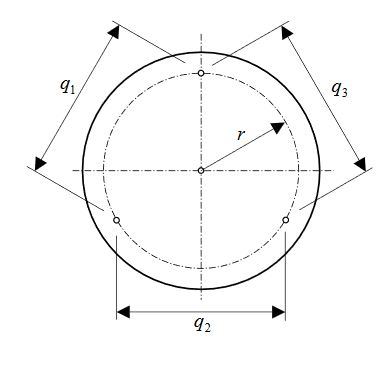
\includegraphics[width=0.5\textwidth]{chapters/lab1/m2topdown}
\caption{Top down view experimental setup for trifilar suspension method.}
\label{fig:mesh2}
\end{figure}
\begin{figure}[H]
\centering
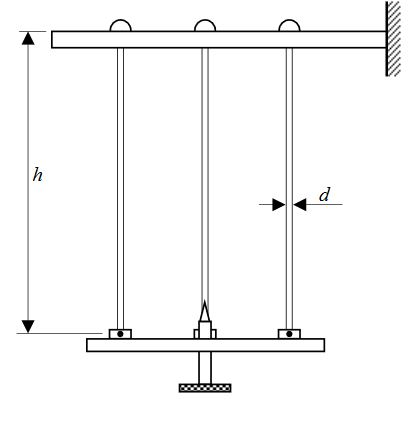
\includegraphics[width=0.5\textwidth]{chapters/lab1/m2}
\caption{Experimental setup for trifilar suspension method.}
\label{fig:mesh2}
\end{figure}

The three readings for the time taken for 40 complete oscillations of the platform carrying the object mass $m$ with oscillations amplitude of approximately 5$^\circ$ and the average period are shown on the table below:
\begin{table}[h!]
\begin{center}
\begin{tabular}{c|c|c|c|}
\cline{2-4}
 &
  \multicolumn{3}{c|}{Trial with Connecting Rod} \\ \cline{2-4} 
 &
  1 &
  2 &
  3 \\ \hline
\multicolumn{1}{|c|}{\multirow{5}{*}{Time (Seconds)}} &
  128.03±0.01 &
  127.94±0.01 &
  \begin{tabular}[c]{@{}c@{}}128.18\\ ±0.01\end{tabular} \\ \cline{2-4} 
\multicolumn{1}{|c|}{} &
  127.87±0.01 &
  \begin{tabular}[c]{@{}c@{}}128.03\\ ±0.01\end{tabular} &
  \begin{tabular}[c]{@{}c@{}}128.25\\ ±0.01\end{tabular} \\ \cline{2-4} 
\multicolumn{1}{|c|}{} &
  \begin{tabular}[c]{@{}c@{}}128.31\\ ±0.01\end{tabular} &
  \begin{tabular}[c]{@{}c@{}}128.12\\ ±0.01\end{tabular} &
  \begin{tabular}[c]{@{}c@{}}128.21\\ ±0.01\end{tabular} \\ \cline{2-4} 
\multicolumn{1}{|c|}{} &
  \begin{tabular}[c]{@{}c@{}}128.06\\ ±0.01\end{tabular} &
  \begin{tabular}[c]{@{}c@{}}128.06\\ ±0.01\end{tabular} &
  \begin{tabular}[c]{@{}c@{}}128.38\\ ±0.01\end{tabular} \\ \cline{2-4} 
\multicolumn{1}{|c|}{} &
  \begin{tabular}[c]{@{}c@{}}128.16\\ ±0.01\end{tabular} &
  \begin{tabular}[c]{@{}c@{}}128.07\\ ±0.01\end{tabular} &
  \begin{tabular}[c]{@{}c@{}}128.28\\ ±0.01\end{tabular} \\ \hline
\multicolumn{1}{|l|}{Average} &
  \begin{tabular}[c]{@{}c@{}}128.086\\ ±0.01\end{tabular} &
  \begin{tabular}[c]{@{}c@{}}128.044\\ ±0.01\end{tabular} &
  \begin{tabular}[c]{@{}c@{}}128.26\\ ±0.01\end{tabular} \\ \hline
\end{tabular}
\caption{The time taken for the loaded platform to complete 40 oscillations.}
\label{tab:5}
\end{center}
\end{table}

\begin{table}[h!]
\begin{center}
\begin{tabular}{c|c|c|c|}
\cline{2-4}
 &
  \multicolumn{3}{c|}{Trial with Connecting Rod} \\ \cline{2-4} 
 &
  1 &
  2 &
  3 \\ \hline
\multicolumn{1}{|c|}{\multirow{5}{*}{Time (Seconds)}} &
  85.14±0.01 &
  84.93±0.01 &
  \begin{tabular}[c]{@{}c@{}}84.53\\ ±0.01\end{tabular} \\ \cline{2-4} 
\multicolumn{1}{|c|}{} &
  85.17±0.01 &
  \begin{tabular}[c]{@{}c@{}}84.78\\ ±0.01\end{tabular} &
  \begin{tabular}[c]{@{}c@{}}84.72\\ ±0.01\end{tabular} \\ \cline{2-4} 
\multicolumn{1}{|c|}{} &
  \begin{tabular}[c]{@{}c@{}}85.07\\ ±0.01\end{tabular} &
  \begin{tabular}[c]{@{}c@{}}84.72\\ ±0.01\end{tabular} &
  \begin{tabular}[c]{@{}c@{}}84.66\\ ±0.01\end{tabular} \\ \cline{2-4} 
\multicolumn{1}{|c|}{} &
  \begin{tabular}[c]{@{}c@{}}85.13\\ ±0.01\end{tabular} &
  \begin{tabular}[c]{@{}c@{}}84.75\\ ±0.01\end{tabular} &
  \begin{tabular}[c]{@{}c@{}}84.54\\ ±0.01\end{tabular} \\ \cline{2-4} 
\multicolumn{1}{|c|}{} &
  \begin{tabular}[c]{@{}c@{}}85.03\\ ±0.01\end{tabular} &
  \begin{tabular}[c]{@{}c@{}}84.65\\ ±0.01\end{tabular} &
  \begin{tabular}[c]{@{}c@{}}84.51\\ ±0.01\end{tabular} \\ \hline
\multicolumn{1}{|l|}{Average} &
  \begin{tabular}[c]{@{}c@{}}85.108\\ ±0.01\end{tabular} &
  \begin{tabular}[c]{@{}c@{}}84.766\\ ±0.01\end{tabular} &
  \begin{tabular}[c]{@{}c@{}}84.592\\ ±0.01\end{tabular} \\ \hline
\end{tabular}
\caption{The time taken for the empty platform to complete 40 oscillations.}
\label{tab:6}
\end{center}
\end{table}

Using the formulae given in the laboratory script to find the time period of oscillation, then the time period for both loaded and empty platform to 3 significant figures calculated to be:
\begin{align}
T_{pm} &= \frac{T_{pm1} + T_{pm2} + T_{pm3}}{120} \notag \\
&= \frac{128.086 + 128.044 + 128.26}{120} \notag \\
&= 3.20 \pm 0.01 seconds \notag \\
T_p  &= \frac{T_{p1} + T_{p2} + T_{p3}}{120} \notag \\
&= \frac{85.108 + 84.766 + 84.592}{120} \notag \\
&= 2.12  \pm 0.01 seconds\notag
\end{align}

The derivation to determine the mass moment of inertia $I$ of an object has been done for us in the laboratory script and the equation $I$ is as shown below:
\begin{equation}
I = \frac{gr^2}{4\pi^2h}\left[T_{pm}^2\left(m_p + m\right) - T_p^2m_p\right] + \frac{3Gd^4}{128\pi h}\left(T_{pm}^2-T_p^2\right)
\end{equation}

Where $g$ is the acceleration due to gravity, $G$ the modulus of rigidity of the steel suspension wires, $m_p$ mass of the empty platform, $m$ is the mass of the object, $h$ is the height of the cable, $T_{pm}$ is the period of the loaded platform, $T_p$ is the period of the empty platform and $r^2$ is given by $\frac{\left(q_1 + q_2+ q_3\right)^2}{27}$. To calculate the mass-moment of inertia of the object, we firstly need to calculate the value of $r^2$:
\begin{align}
r^2 &= \frac{(0.1313 + 0.1312 + 0.1314)^2}{27} \notag \\
&= 0.005746563 \notag \\
\delta r^2 &= \frac{2*(q_1 + q_2 + q_3)}{27}(\delta (q_1 + q_2 + q_3)) \notag \\
&=\frac{2*(0.1313+0.1312+0.1314)}{27}(\delta (0.003)) \notag \\
&= 8.75 \times 10^{-5} \notag \\
r^2 &= 0.005746563 \pm 8.75 \times 10^{-5} m^2 \notag
\end{align}
Substituting the value $r^2$ above into equation 5 along with other values that are required to calculate mass-moment of inertia, then the mass-moment of inertia and its uncertainty values are calculated to be:
\begin{align}
I &= \frac{0.005746563*9.794}{4*\pi^2*1.87}\left[3.202325^2\left(1.997 + 2.65\right) - 2.120255^2*1.997\right] \notag \\
&\qquad+ \frac{3*80 \times 10^9*0.00132^4}{128*\pi*1.87}\left(3.20325^2-2.12055^2\right) \notag \\
I &= 0.035 kg.m^2 \notag \\
\delta I &= \pm \abs{\left(\dfrac{3\left(T_{pm}^2-T_p^2\right)Gd^3}{32{\pi^2}h}\right)(\delta d)} \notag \\
&\qquad + \abs{\dfrac{\left(T_{pm}^2\left(m_p+m\right)-T_p^2m_p\right)r^2}{4{\pi^2}h}(\delta g)} \notag \\
&\qquad + \abs{\left(-\dfrac{3d^4\left(T_{pm}^2-T_p^2\right)G}{128{\pi}h^2}-\dfrac{g\left(T_{pm}^2\left(m_p+m\right)-T_p^2m_p\right)r^2}{4{\pi^2}h^2}\right)(\delta h) } \notag \\
&\qquad + \abs{\left(\dfrac{gT_{pm}^2r^2}{4{\pi^2}h}\right)(\delta m)} +  \abs{\dfrac{3d^4GT_{pm}}{64{\pi}h}+\dfrac{g\left(m_p+m\right)r^2T_{pm}}{2{\pi}^2h}(\delta T_{pm})}\notag \\
&\qquad + \abs{\left(-\dfrac{\left(3{\pi}d^4G+32gm_pr^2\right)T_p}{64{\pi^2}h}\right)(\delta T_p)} + \abs{\left(\dfrac{g\left(T_{pm}^2-T_p^2\right)r^2}{4{\pi^2}h}\right)(\delta m_p)} \notag \\
&\qquad + \abs{\left(\dfrac{g\left(T_{pm}^2\left(m_p+m\right)-T_p^2m_p\right)r}{2{\pi^2}h}\right)(\delta r)} \notag \\
\delta I &= 6.60\times10^{-4} \notag \\
I &= 0.035 \pm 6.60\times10^{-4} kg.m^2 \notag
\end{align}